%%%%%%%%%%%%%%%%%%%%%%%%%%%%%%%%%%%%%%%%%%%%%%%%%%%%%%%%%%%%%%%%%%%%%%%%%%%%
%    This LaTeX source was automatically generated by outlinebeamer.pl     %
%                                                                          %
%   Remember that most changes should be made to the outline source file   %
% changes to this file will be overwritten when the file gets regenerated  %
%                                                                          %
%                  outlinebeamer - Outline Beamer Class Presentation Maker %
%                                    http://outlinebeamer.sourceforge.net/ %
%%%%%%%%%%%%%%%%%%%%%%%%%%%%%%%%%%%%%%%%%%%%%%%%%%%%%%%%%%%%%%%%%%%%%%%%%%%%
%\documentclass{beamer}
\documentclass{beamer}

\usetheme{Copenhagen}
\usecolortheme{default}

\newcommand{\Code}[1]{\textsf{#1}}
\newcommand{\cello}{\textsf{Cello}}
\newcommand{\enzo}{\textsf{Enzo}}
\newcommand{\code}[1]{\texttt{#1}}
\newcommand{\us}[1]{\color{blue}{#1}}
\newcommand{\them}[1]{\color{red}{#1}}
\newcommand{\newus}[1]{\color{magenta}{#1}}
\newcommand{\good}{\textcolor{green}{\smiley}}
\newcommand{\bad}{\textcolor{red}{\frownie}}
\newcommand{\colorcode}[1]{\textcolor{blue}{\code{#1}}}
\newcommand{\itemnum}[1]{\item<#1>}

%========================================================================
% UNCOMMENT TO PRINT
%========================================================================

 \newcommand{\enhance}[1]{}
 \newcommand{\enhancebf}[2]{\textbf{#2}}
 \newcommand{\enhanceus}[1]{\color{blue}}
 \newcommand{\enhancenewus}[1]{\color{magenta}}
 \newcommand{\enhancethem}[1]{\color{red}}
\newcommand{\ENHANCE}[1]{
 \temporal<#1>{\color{lightgray}}{\color{black}}{\color{gray}}}

%========================================================================
% UNCOMMENT FOR TALK:
%========================================================================

% \newcommand{\enhance}[1]{\temporal<#1>{\color{lightgray}}{\color{black}}{\color{black}}}
% \newcommand{\enhancebf}[2]{\enhance{#1}\textbf{#2}}
% \newcommand{\enhanceus}[1]{\temporal<#1>{\color{lightgray}}{\color{blue}}{\color{blue}}}
% \newcommand{\enhancenewus}[1]{\temporal<#1>{\color{lightgray}}{\color{magenta}}{\color{magenta}}}
% \newcommand{\enhancethem}[1]{\temporal<#1>{\color{lightgray}}{\color{red}}{\color{red}}}
%\newcommand{\ENHANCE}[1]{
% \temporal<#1>{\color{lightgray}}{\color{black}}{\color{black}}}
%========================================================================


% \def\enhanceus<#1>{%
%  \temporal<#1>{\color{lightgray}}{\color{blue}}{\color{blue}}}
% \def\enhancenewus<#1>{%
%  \temporal<#1>{\color{lightgray}}{\color{magenta}}{\color{magenta}}}
% \def\enhancethem<#1>{%
%  \temporal<#1>{\color{lightgray}}{\color{red}}{\color{red}}}


%\includeonly{array}


%======================================================================
\title[The \cello\ Project]
      {The \cello\ Project \\ \small{\enzo: The Next Generation}}
\author[James Bordner]{\small Laboratory for Computational Astrophysics \\ Center for Astrophysics and Space Sciences \\San Diego Supercomputer Center \\ University of California, San Diego \\ \ \\ James Bordner}
\date{September 24, 2009}
\begin{document}
\frame{\titlepage}

%========================================================================
% UNCOMMENT FOR TALK
% COMMENT FOR PRINT
%========================================================================
%\frame{\footnotesize
%\tableofcontents}
% \AtBeginSection[]
%{
%%------------------------------------------------------------------------
%  \begin{frame}<beamer>
%\footnotesize
%   \tableofcontents[currentsection]
%%    \tableofcontents[currentsection]
%  \end{frame}
%}
%========================================================================

%========================================================================
\section{Introduction}
%========================================================================

% \include{outline}

%------------------------------------------------------------------------
\subsection{Goals}
%------------------------------------------------------------------------
\begin{frame}[fragile] \frametitle{Project Goals}
   \begin{itemize}
      \item\enhance{1} \enzo: The Next Generation
      \item\enhance{2} Computational astrophysics code for next 10+ years
      \item\enhance{3} Scalable to largest available platforms: O($10^{5+}$)  cores
      \item\enhance{4} Easy modify, enhance, adapt, maintain
      \item\enhance{5} Easy to define and run new problems
      \enhance{6}\item Capable of advancing science knowledge
   \end{itemize}
\end{frame}



%------------------------------------------------------------------------
\subsection{Scope}
%------------------------------------------------------------------------

%------------------------------------------------------------------------
    \begin{frame}[fragile] \frametitle{Target Classes of Users}
      \begin{itemize}
        \item \enhancebf{1}{Graduate students}
        \begin{itemize}
          \item \enhance{1}easy to define problem, run, and analyze
          \item \enhance{1}minimal software-, hardware-, or method-related ``gotcha's''
        \end{itemize}
        \item \enhancebf{2}{Physics experts}
        \begin{itemize}
          \item \enhance{2}deep control of physics parameters
          \item \enhance{2}ability to solve a wide range of problems
        \end{itemize}
        \item \enhancebf{3}{Numerical experts}
        \begin{itemize}
          \item \enhance{3}deep control of method parameters
          \item \enhance{3}easy to incorporate new methods
        \end{itemize}
        \item \enhancebf{4}{Computing experts}
        \begin{itemize}
          \item \enhance{4}deep control of data structures
          \item \enhance{4}AMR, parallelization, data distribution, array layout
        \end{itemize}
      \end{itemize}
\end{frame}

%------------------------------------------------------------------------
    \begin{frame}[fragile] \frametitle{Target Classes of Problems}

      \begin{itemize}
        \item \enhance{1}\textbf{Unigrid (turbulence)}
        \begin{itemize}
          \item  \enhance{1}parallelizes fully
          \item  \enhance{1}\enzo\ does well, but still room for improvement
        \end{itemize}
        \item \enhance{2}\textbf{``Typical'' AMR (cosmology)}
        \begin{itemize}
	   \item \enhance{2}\enzo\ does ok, but has scaling issues
	   \item \enhance{2}load-balancing, memory usage, etc.
        \end{itemize}
        \item \enhance{3}\textbf{``Deep'' AMR (star formation)}
        \begin{itemize}
          \item \enhance{3}most difficult to parallelize effectively
          \item \enhance{3}\enzo\ has done deep runs, but not without difficulty
          \item \enhance{3}floating-point precision and integer range issues
        \end{itemize}
        \item \enhance{4}\textbf{Ensembles (parameter studies)}
        \begin{itemize}
           \item \enhance{4}Inter-simulation inline analysis
        \end{itemize}
 
      \end{itemize}
\end{frame}



%------------------------------------------------------------------------
\subsection{Issues}
%------------------------------------------------------------------------

%------------------------------------------------------------------------
\begin{frame}[fragile] \frametitle{Petascale performance Issues}
   \begin{itemize}
      \item \enhance{1}Parallel task control
      \begin{itemize}
          \item \enhance{1}Large enough to be efficient
          \item \enhance{1}Small enough for sufficient parallelism
      \end{itemize}
      \item \enhance{2}Parallel task scheduling
      \begin{itemize}
          \item \enhance{2}Static scheduling with dynamic load balancing
          \item \enhance{2}Dynamic scheduling with job migration
      \end{itemize}
      \item \enhance{3}Load balancing across nodes / cpus / cores
      \item \enhance{4}Global synchronization
      \item \enhance{5}Software resiliency / fault tolerance
      \item \enhance{6}Checkpoint / restart
   \end{itemize}
\end{frame}


%========================================================================
\section{Software Design}
%========================================================================

%------------------------------------------------------------------------
\subsection{Input files}
%------------------------------------------------------------------------

\begin{frame}[fragile] \frametitle{Input Files}
\begin{itemize}
   \item\enhance{1}Important: point-of-contact between user and application
   \item\enhance{2}Limiting factor in usability and power of the application
   \item\enhance{3}Maximize expressibility; minimize complexity
   \item\enhance{4}Approach: remove ``\code{ProblemType}'' parameter
   \begin{itemize}
      \item\enhance{5}Restricts scope of problems solved
      \item\enhance{6}Problem solved not obvious from input file
   \end{itemize}
   \item\enhance{7}Overall code size will be much smaller
   \begin{itemize}
      \item\enhance{7} $\approx$\code{20\%} of \enzo\ C++ functions contain ``Initialize''!
   \end{itemize}
   \item\enhance{8}Can fake it with e.g.~\code{\#include "implosion.enzo"}
\end{itemize}
\end{frame}

\begin{frame}[fragile] \frametitle{Input Files}
\begin{itemize}
   \item\enhance{1}Helpful to have more powerful syntax and grammar
  \begin{block}{}\footnotesize\enhance{2}
      \verb+Method ppm {+ \\
      \verb+   diffusion = false;+ \\
      \verb+}+
   \end{block}
   \item\enhance{3}Requires more data types
  \begin{block}{}\footnotesize
  \begin{tabular}{ll}
	\enhance{4}Scalar expressions &\enhance{4} \code{exp(cos(x) + sin(y))} \\
	\enhance{4}Logical expressions &\enhance{4} \code{x*x + y*y <= 1} \\
       \enhance{4} Lists  &\enhance{4} \code{[1.9e6, x <= y, "omp"]}
   \end{tabular}
   \end{block}
   \item\enhance{5} Input file parsing not overly difficult
   \begin{itemize}
      \item\enhance{5} \code{flex} and \code{bison} tools
   \end{itemize}
\end{itemize}
\end{frame}

%------------------------------------------------------------------------
    \begin{frame}[fragile] \frametitle{Draft Input File: Implosion}
 \footnotesize
\begin{block}{Implosion: domain, grid, and field parameters}
\begin{verbatim}
# Define the domain to be the 2D box 0 < x,y < 0.3

Domain { range = [0.0, 0.3, 0.0, 0.3] } 
                                
# The grid is a "unigrid" array of 400 cells
 
Grid { size = [400,400]; parallel = ["mpi"] }

# Define some field properties
                                
Field pressure { floor = 1.0e-6 }
Field density  { floor = 1.0e-6 }
\end{verbatim}
\end{block}
\end{frame}

%------------------------------------------------------------------------
\begin{frame}[fragile] \frametitle{Draft Input File: Implosion}
\footnotesize
\begin{block}{Implosion: method parameters and boundary conditions}
\begin{verbatim}
# PPM hydrodynamics

Method ppm {
   gamma     = 1.4;
   courant   = 0.8;
   diffusion = true;
   flattening = true;
   steepening = true;
}

# Define boundary conditions

Boundary { type = "reflecting" }
\end{verbatim}
\end{block}
\end{frame}

%------------------------------------------------------------------------
\begin{frame}[fragile] \frametitle{Draft Input File: Implosion}
 \footnotesize
\begin{block}{Implosion: Initial conditions and stopping criteria}
\begin{verbatim}
# Initial conditions

Initial {
   density  = [1.0, x + y >= 0.15, 0.125];
   pressure = [1.0, x + y >= 0.15, 0.14];
   velocity_x = 0;
   velocity_y = 0;
}

# Stopping criteria

Stopping {
   time  = 2.5;
   cycle = 20000;
}
\end{verbatim}
\end{block}
\end{frame}


%------------------------------------------------------------------------
\subsection{Software components}
%------------------------------------------------------------------------

%@@@@@@@@@@@@@@@@@@@@@@@@@@@@@@@@@@@@@@@@@@@@@@@@@@@@@@@@@@@@@@@@@@@@@@@
\chapter{Components} \label{c:components}
%@@@@@@@@@@@@@@@@@@@@@@@@@@@@@@@@@@@@@@@@@@@@@@@@@@@@@@@@@@@@@@@@@@@@@@@

\centerline{\includegraphics{uml/core-components.1}}

Core components

\begin{itemize}
\item Control
\item Problem
\item Method
\item Data
\item Storage
\end{itemize}

\begin{itemize}
\item Parallel
\item Parallel:MPI
\item Parallel:OMP
\end{itemize}


   This chapter describes the design of \cello\ at the component
   level.  Each component is described, including the component interface and dependencies on other components.  Class-level design of each component is described in \S\ref{c:classes}.


Input is in the form of a text file that specifies
   parameter values.  The input file may optionally include other
   input files.

   Parameters are organized into functional groups, which are described
   in more detail in subsequent sections.

\begin{description}

 \item [Control (\S\ref{s:component-control}): ] Control parameters specify the
 high-level parameters, as well as controling interactions between
 other components such as Parallel, Method, and Datastructure.  May
 include sequence and interaction of physics modules, parallel dynamic
 load-balancing, refinement criteria, numerical floors and limits,
 dynamic refinement in subregions, etc.

 \item [Physics (\S\ref{s:component-physics}): ] Physics parameters are used to
 define which physics is enabled---such as self-gravity,
 hydrodynamics, cosmological expansion, etc.  They also define any
 parameters associated with the physics of the problem being solved,
 such as cosmological parameters and the gravitational constant.
 Physics parameters define what physics to simulate in the
 computational universe.

 \item [Problem (\S\ref{s:component-problem}): ] Problem parameters include
 the domain extents, boundary and initial conditions.

 \item [Units (\S\ref{s:component-units}): ] Units parameters define the problem
 units, as well as scalings for computation if different.  Allows for
 ``variable'' scaling (e.g.~to keep values near unity to avoid under-
 or overflow) and quantization of scaling factors (e.g.~scale by $2^k$
 to avoid loss of precision).

 \item [Domain (\S\ref{s:component-domain}): ] Domain parmeters include extents
 and dimensionality.

 \item [Region (\S\ref{s:component-region}): ] A region is a subset of the
 domain.  Regions are used whenever problem characteristics,
 datastructure behavior, or physics computations vary between
 different spacial regions.  A region may include the entire
 domain.

 \item [Field (\S\ref{s:component-field}): ] Field parameters define all fields
 used in the computation, including their names, and whether they are
 scalar or vector fields.  Field parameters associate the name,
 datastructure, and units.

 \item [Matter (\S\ref{s:component-matter}): ] Matter defines properties of
 different types of matter used in the simulation, such as gas
 constants, dark matter, etc.

 \item [Method (\S\ref{s:component-method}): ] Method parameters specify the
 method to use for each physics component, and any associated
 method-specific parameters.  This also includes how methods are to be
 coupled together.  Method parameters define how to simulate the
 physics in the computational universe.

 \item [Data (\S\ref{s:component-data}): ] Data parameters include listing which
 data structures to use (unigrid, SAMR, particles, subblocks, etc.),
 as well as all associated parameters (unigrid resolution, SAMR mesh
 levels, particle attributes, array subblock size control, ghost zone
 width and longevity, etc.)  Datastructure parameters define how to
 represent the continuous (infinite dimensional) problem and physics
 as a computationally solveable (finite dimensional) discrete problem.
 Some parameters, such as subblock size, may affect performance but
 not the solution.  Data parameters include Hierarchy, Particle,
 Array, and Patch parameters.

 \item [Parallel (\S\ref{s:component-parallel}): ] Parallelism parameters
 specify which levels to parallelize (simulations, patches, and
 subblocks), how to parallelize each level (MPI-1 2-sided, MPI-2
 1-sided, OpenMP, UPC), and lower-level parameters (buffering,
 blocking or nonblocking, patch-to-processor mapping,
 subblock-to-thread mapping, etc.)

 \item [Performance (\S\ref{s:component-performance}): ] Performance
 self-monitoring and optimization parameters.

 \item [Monitor (\S\ref{s:component-monitor}): ] Monitor parameters control what
 and when to output user-readable summary information about the
 running application, such as status summary, progress, warnings,
 errors, and performance information.

 \item [Storage (\S\ref{s:component-storage}): ] The \code{Storage}
 component controls what, when, and how to input and output
 large-scale data, primarily data fields.

 \item [Portal (\S\ref{s:component-portal}): ] Portal parameters control
  how to interface with external applications.

 \item [Recover (\S\ref{s:component-recover}): ] The \code{Recover}
 package controls how to detect errors, and what to do if errors are
 detected.

\end{description}

\begin{tabbing}
xxx\=xxx\=xxx\=xxx\=xxxxxxxx\= \kill
\ref{s:component-control} \>      \code{Control}     \>\>\>\> \textit{Manages everything}  \\
\ref{s:component-parameters} \>\>    \code{Parameters}    \>\>\> \textit{Reading and accessing all parametrs} \\
\ref{s:component-parallel}  \>\>    \code{Parallel}      \>\>\> \textit{Manages multiple parallelization levels and technologies} \\
\ref{s:component-recover}  \>\>    \code{Recover}      \>\>\> \textit{Detects, evaluates, and recovers from hardware or software errors} \\
\ref{s:component-portal}  \>\>    \code{Portal}        \>\>\> \textit{Controls access to internal state and data by external entities} \\
\ref{s:component-performance}  \>\>    \code{Performance}   \>\>\> \textit{Measures and allows other components to access performance data} \\
\ref{s:component-monitor}  \>\>    \code{Monitor}       \>\>\> \textit{Enables users to monitor the state and progress of the simulations} \\
\ref{s:component-simulation}  \>      \code{Simulation}  \>\>\>\> \textit{Description of a single astrophysics simulation} \\
\ref{s:component-problem}  \>\>    \code{Problem}       \>\>\> \textit{Declaration of what to simulation} \\
\ref{s:component-domain}  \>\>\>  \code{Domain}          \>\> \textit{The problem domain} \\
\ref{s:component-field}  \>\>\>  \code{Field}           \>\> \textit{A scalar or vector field} \\
\ref{s:component-boundary}  \>\>\>  \code{Boundary}        \>\> \textit{Boundary conditions} \\
\ref{s:component-initial}  \>\>\>  \code{Initial}         \>\> \textit{Initial conditions} \\
\ref{s:component-region}  \>\>\>\>\code{Region}            \> \textit{A subset of the domain} \\
\ref{s:component-physics}  \>\>    \code{Physics}       \>\>\> \textit{A physical law or process and associated parameters} \\
\ref{s:component-units}  \>\>\>  \code{Units}           \>\> \textit{Units used for user and computational fields} \\
\ref{s:component-material}  \>\>\>  \code{Material}        \>\> \textit{Type of matter, e.g.~gas, H+, e-, dark matter} \\
\ref{s:component-method}  \>\>    \code{Method}        \>\>\> \textit{Numerical method for evolving a physical law or laws} \\
\ref{s:component-analysis}  \>\>    \code{Analysis}      \>\>\> \textit{Numerical method for post-processing data} \\
\ref{s:component-data}  \>\>    \code{Data}          \>\>\> \textit{Numerical representation of data fields} \\
\ref{s:component-hierarchy}  \>\>\>  \code{Hierarchy}       \>\> \textit{AMR hierarchy} \\
\ref{s:component-level}  \>\>\>  \code{Level}           \>\> \textit{Uniform resolution component of an AMR hierarchy} \\
\ref{s:component-patch}  \>\>\>  \code{Patch}           \>\> \textit{Rectangular grid of cells of uniform resolution in a hierarchy} \\
\ref{s:component-box}  \>\>\>\>\code{Box}               \> \textit{Rectangular box with position and size} \\
\ref{s:component-array}  \>\>\>\>\code{Array}             \> \textit{Array of floating-point values} \\
\ref{s:component-IO}  \>\>\code{IO}            \>\>\> \textit{Description of what data to output, how, and when}
\end{tabbing}

%-----------------------------------------------------------------------

%=======================================================================
\section{Control parameters} \label{s:control}
%=======================================================================

Given Physics, Algorithms, and Data structures, specify the top-level
sequencing and properties of the simulation.  For example, ordering of
physics modules, whether to do hierarchical time-stepping, up to what
level, whether to sub-cycle some physics, etc. [Is this a useful
category?]  Also include things like floors and limits(?), and IO
dumps

Global simulation control.

Output types and parameters

\begin{itemize}
\item checkpoint (dump all)
\item output (specific fields)
\item movies (type and rate)
\item analysis (type of analysis, rate)
\item level of output (files for timestep, time, etc.)
\end{itemize}

%-----------------------------------------------------------------------
\subsection{Use Cases}
%-----------------------------------------------------------------------
%-----------------------------------------------------------------------
\subsection{Parameters}
%-----------------------------------------------------------------------



%=======================================================================
\section{Physics parameters} \label{s:physics}
%=======================================================================

Specify physics modules and physics parameters, including
hydrodynamics, self-gravity, gravitational constant, imposed gravity,
chemistry, cosmological expansion, star formation, etc.  Physics is in
the problem domain.

Specify physics components

\begin{itemize}
\item hydrodynamics
\item  cosmological expansion
\item self-gravity
\end{itemize}

%-----------------------------------------------------------------------
\subsection{Use Cases}
%-----------------------------------------------------------------------
%-----------------------------------------------------------------------
\subsection{Parameters}
%-----------------------------------------------------------------------

%=======================================================================
\section{Units parameters} \label{s:units}
%=======================================================================

 Specify units and optional scalings for individual
 fields.  [Merge units with Control?] [Merge scaling with Fields?] 
 [Dynamic scaling, e.g.~to keep average of all fields near one.]

%-----------------------------------------------------------------------
\subsection{Use Cases}
%-----------------------------------------------------------------------
%-----------------------------------------------------------------------
\subsection{Parameters}
%-----------------------------------------------------------------------

%=======================================================================
\section{Problem Component} \label{s:component-problem}
%=======================================================================

Problem parameters specify the setup of the physical problem,
including initial conditions of relevant data fields and boundary
conditions.

  dimensionality
  domain extents
  initial conditions (materials, regions, input)
 boundary conditions (periodic, in-/out-flow, specified, dynamic)

Problem parameters include initial conditions and boundary conditions.

Different types of boundary conditions are supported, including
periodic, in- and out-flow, specified, and dynamic.  Different
boundary conditions can be specified for the entire domain, on
separate faces, on subregions of faces, or on specific zones.
Different boundary conditions can be specified for different fields.
%-----------------------------------------------------------------------
\subsection{Use Cases}
%-----------------------------------------------------------------------

\begin{verbatim}
   problem {
      boundary {
         x:lower = reflecting
         x:upper = { type = reflecting }
         y       = { type = periodic }
         z       = { type = inflow,  value = 1.0 }
         z       = { outflow, 1.0 }
      }
   }
\end{verbatim}

\begin{verbatim}
   XM = boundary { x = domain:lower[0] }
   XP = boundary { x = domain:upper[0] }
   YM = boundary { y = domain:lower[1] }
   YP = boundary { y = domain:upper[1] }
   ZM = boundary { z = domain:lower[2] }
   ZP = boundary { z = domain:upper[2] }
   field {
      name = "density"
      value(XM) = 0
      value(XP) = 0
      value(YM) = value (YP)
      value(ZM) = +t
      value(ZM) = -t
   }
\end{verbatim}

%-----------------------------------------------------------------------
\subsection{Parameters}
%-----------------------------------------------------------------------

%=======================================================================
\section{Data Component} \label{s:component-data}
%=======================================================================

Specify low-level datastructures (fields and particles) and their
parameters.

Use chunked field storage \\
Field chunk size or range


%=======================================================================
\subsection{Arrays}

%=======================================================================
\subsection{Fields}

%=======================================================================
\subsection{Particles}

%=======================================================================
\subsection{Structured Adaptive Mesh Hierarchies}

%=======================================================================
\subsection{Octree}


%=======================================================================
\section{Domain Component} \label{s:component-domain}
%=======================================================================

The \code{domain} function is used to specify properties of the
domain.  Domains are boxes aligned with the axes of the computational
coordinate system, and are uniquely determined by the spacial
dimension, and the lowest and highest points in the domain.

%-----------------------------------------------------------------------
\subsection{Use Cases}
%-----------------------------------------------------------------------

\begin{verbatim}
   domain { 
      dimension = 3
      lower     = <-3e9,-3e9,-3e9>
      upper     = <3e9,3e9,3e9>
   }
\end{verbatim}

\begin{verbatim}
   domain { 3, <-3e9,-3e9,-3e9>, <3e9,3e9,3e9> }  // Implicit ordering
\end{verbatim}

\begin{verbatim}
   domain { 
      dimension = 3
      upper     = 3e9        // expand scalar to vector
      lower     = -upper     // parameters can be accessed as values
   }
\end{verbatim}

Include errors.

%-----------------------------------------------------------------------
\subsection{Parameters}
%-----------------------------------------------------------------------

 \todo\ \textit{Decide: allow defaults?  allow optional parameters?  Special
 \code{OPT\_} prefix for optional parameters?  Write out explicit copy
 of input file?}

The \code{domain} function has three parameters

\begin{tabular}{lll} \\
Name & Type & Restrictions \\ \hline
\code{dimension} & Scalar & $1-3$ \\
\code{lower}     & Vector & length = \code{dimension} \\
\code{upper}     & Vector & length = \code{dimension}, \code{upper} $>$ \code{lower}
\end{tabular}

Lower and upper points are given in units given by \code{units},
described in \S\ref{s:units}.

%-----------------------------------------------------------------------
\subsection{Restrictions}
%-----------------------------------------------------------------------

\begin{enumerate}
\item The dimension must be 1, 2, or 3.
\item The number of coordinates in both lower and upper points must equal the dimension.
\item Each coordinate of the lower point must be strictly greater than the corresponding coordinate of the upper point.
\end{enumerate}




%=======================================================================
\section{Region Component} \label{s:component-region}
%=======================================================================

Specify partitions of the domain into regions.  Each region contains
different materials with different properties.  Example partitions may
be half-planes, spheres, boxes, or specified using a file containing a
zone bit mask.  Default is region 0, first region is region 1, etc.
Use solid modeling representations?

%-----------------------------------------------------------------------
\subsection{Use Cases}
%-----------------------------------------------------------------------

\begin{verbatim}
   region {
      x + y + z < 0.5
   }
\end{verbatim}

\begin{verbatim}
   BOX = region {
      (x > 0) &&
      (x < 1) &&
      (y > 0) && (y < 1) &&
      (z > 0) && (z < 1)
   }
\end{verbatim}

\begin{verbatim}
   region {
      union {
         region {BOX, translate = 0.0*x, scale = 0.1}
         region {BOX, translate = 0.1*x, scale = <0.1,0.1,0.1>}
         region {BOX, translate = 0.2*x, scale = 0.1}
      }
   }
\end{verbatim}

\begin{verbatim}
   region {
      x = domain:lower[0]
   }
\end{verbatim}

\begin{verbatim}
   region {
      x*x + y*y + z*z < 1
   }
\end{verbatim}

\begin{verbatim}
   region {
      bitmask = "filename.hdf5"
   }
\end{verbatim}


%-----------------------------------------------------------------------
\subsection{Parameters}%
-----------------------------------------------------------------------


%=======================================================================
\section{Field Component} \label{s:component-field}
%=======================================================================

Scalar and vector fields for each material, such as
 density, energy, velocity, etc.  [Merge with Materials?]  Specify
 values, or input from files.

%-----------------------------------------------------------------------
\subsection{Use Cases}
%-----------------------------------------------------------------------
\begin{verbatim}
   field {
      name     = "density"
      name     = "rho"
      type     = scalar
      location = center
   }
   field {
      name     = "velocity"
      name     = "u"
      type     = vector
      location = center
   }
   field {
      name     = "temperature"
      name     = "T"
      type     = scalar
      location = center
   }
   field {
      name     = "B"
      type     = computed
      location = face
   }
\end{verbatim}

%-----------------------------------------------------------------------
\subsection{Parameters}
%-----------------------------------------------------------------------

%=======================================================================
\subsection{\code{Units} Component} \label{ss:component-units}
%=======================================================================

 Specify units and optional scalings for individual
 fields.  
 \note{Dynamic scaling, e.g.~to keep average of all fields near one.}

%-----------------------------------------------------------------------
\subsubsection{Use Cases}
%-----------------------------------------------------------------------
%-----------------------------------------------------------------------
\subsubsection{Parameters}
%-----------------------------------------------------------------------

%=======================================================================
\subsection{\code{Matter} Component} \label{ss:component-matter}
%=======================================================================

 Specify units and optional scalings for individual
 fields.  
 \note{Dynamic scaling, e.g.~to keep average of all fields near one.}

%-----------------------------------------------------------------------
\subsubsection{Use Cases}
%-----------------------------------------------------------------------

%-----------------------------------------------------------------------
\subsubsection{Parameters}
%-----------------------------------------------------------------------

\begin{verbatim}
   Matter {
      type = dark
   }
\end{verbatim}

\begin{verbatim}
   Matter {
      type  = gas_ideal
      gamma = 1.4
   }
\end{verbatim}


\subsection{ Field  Component}
Scalar fields on an Array or Mesh hierarchy

A Field represents a discretized scalar field. A Field is typically
discretized on an AMR hierarchy, but can be accessed at the Array or a
Block levels as well. In addition to the array of elements, a Field
includes an identifier for the field, the location of the field values
with respect to computational cells (cell centered, face-centered,
etc.), the index into the Block or Array of the field, optional
minimum or maximum allowed values, units, and user-defined tags.

Attributes:

\begin{tabular}{ll}
    \code{name}        & String defining the field's name, e.g. "density", "velocity-x", etc. \\
    \code{id} 	& Integer identifying the Field \\
    \code{array} &	Array containing Field values for the containing Patch \\
    \code{index} &	Index of the specific array in the 4D Array \\
    \code{position} &	cell position, defined as (0,0,0) <= (px,py,pz) <= (1,1,1). (.5,.5,.5)=cell centered \\
    \code{min} &	minimum allowed value for the Field \\
    \code{max} &	maximum allowed value for the Field \\
    \code{min\_action} &	what should be done if Field goes below min (e.g. 1: set to min, 2: warning, 4: error, g: retry with smaller timestep, etc.) \\
    \code{max\_action} &	what should be done if Field goes above max
\end{tabular}

A set of Fields defined on a Block, along with groups of Particles
associated with the block, are the main input to (and output from)
Methods. Methods have access to the Field's values, size, cell
position, units, tags, limits, etc.

Actual Field objects are stored in the Mesh Patch object. Patch objects
also contain associated Particle objects, and a Box object defining
the Patch's extents and position.  List of fields


Field supporting classes

Field operations
Field hierarchy
Structure
Descriptions
Field class
Attributes
Functions
Usage

Issues:

\begin{itemize}
\item What operations are the responsibility of Field versus Array,
  Task, Patch, etc.
\item see below: Field stores only global properties of field, not
  actual data
\item How to store global attributes (name, index, min, max, position,
  etc.) versus non-global (values)
\item Single global Field object for each field
\item Fields don't store actual Arrays, Patches do--Field only stores
  Array index.
\end{itemize}

%=======================================================================
\section{Matter Component} \label{s:component-matter}
%=======================================================================

 Matter defines properties of matter, such as the matter type (baryonic
 or dark matter), and gas constants.

%-----------------------------------------------------------------------
\subsection{Use Cases}
%-----------------------------------------------------------------------

\begin{verbatim}
   Matter {
      type = dark
   }
\end{verbatim}

\begin{verbatim}
   Matter {
      type  = gas_ideal
      gamma = 1.4
      region { (x < 0) || (x > 1) }
   }
\end{verbatim}
%-----------------------------------------------------------------------
\subsection{Parameters}
%-----------------------------------------------------------------------

%=======================================================================
\section{Method Component} \label{s:component-method}
%=======================================================================

  Defines how to simulate the physics in the computational universe.
  A \code{Method} specifies the numerical method to use, which
  \code{Field}s are involved, and any associated method-specific
  parameters.  Sequencing and coupling of \code{Method}s is defined in
  \code{Problem} and implemented in \code{Control}.  Analysis and
  visualization are considered \code{Method}s as well.

\begin{itemize}
\item HD
\item MHD
\item RHD
\item cooling
\item gravity
\end{itemize}

Specify algorithms and their parameters.

HD dual-energy

HD steepening
HD flattening
HD diffusion

Timestepping


\begin{itemize}
\item PPM hydro (dual-energy, etc.)
\item gravity solver (FAC, smoother, levels, etc.)
\end{itemize}

%-----------------------------------------------------------------------
\subsection{Use Cases}
%-----------------------------------------------------------------------
%-----------------------------------------------------------------------
\subsection{Parameters}
%-----------------------------------------------------------------------

%=======================================================================
\subsection{Method:Hydro subcomponent}

%=======================================================================
\subsection{Method:Gravity subcomponent}

%=======================================================================
\subsection{Method:Cooling subcomponent}

%=======================================================================
\subsection{Method:Chemistry subcomponent}

%=======================================================================
\subsection{Method:MHD subcomponent}

%=======================================================================
\subsection{Method:RT subcomponent}

%=======================================================================
\subsection{Analysis subcomponent} \label{ss:component-analysis}
%=======================================================================

 Specify the algorithms and algorithm parameters to use for analysis
 and visualization.

%=======================================================================
\subsection{Visualization subcomponent} \label{ss:component-visualization}
%=======================================================================


%=======================================================================
\section{AMR Component} \label{s:component-amr}
%=======================================================================

Specify data structures and data structure parameters for distributed
AMR hierarchies, such as number of mesh levels, grid patch properties,
rebuild algorithm, dynamic load balancing, refinement criteria, etc.

Hierarchy
Array


\begin{itemize}
\item hierarchy
\begin{item}
\item min\_levels 
\item max\_levels 
\end{item}
\item level
\item grid
\begin{itemize}
\item min\_size
\item max\_size
\item max\_aspect
\item quantum
\end{itemize}
\end{itemize}

\centerline{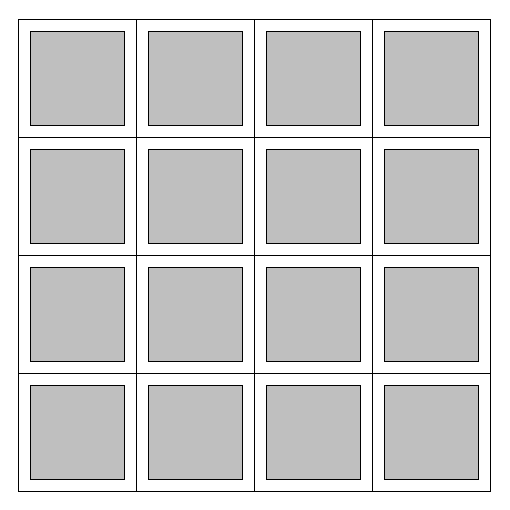
\includegraphics[width=1.8in]{amr4-1.eps} \ \
            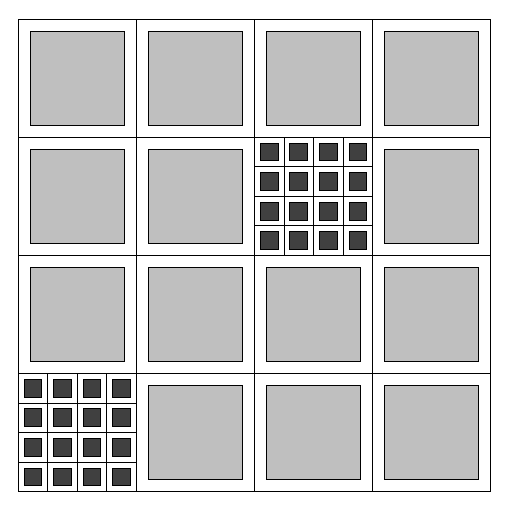
\includegraphics[width=1.8in]{amr4-2.eps} \ \
            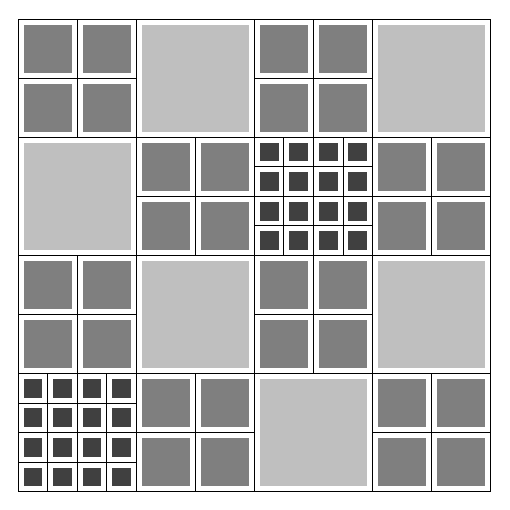
\includegraphics[width=1.8in]{amr4-3.eps}}

\centerline{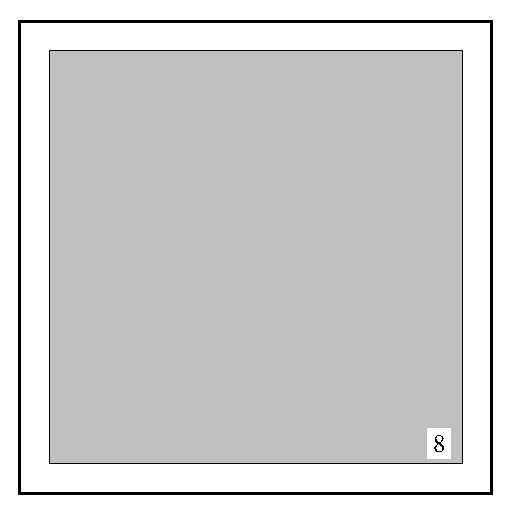
\includegraphics[width=1.8in]{amr2-1.eps} \ \
            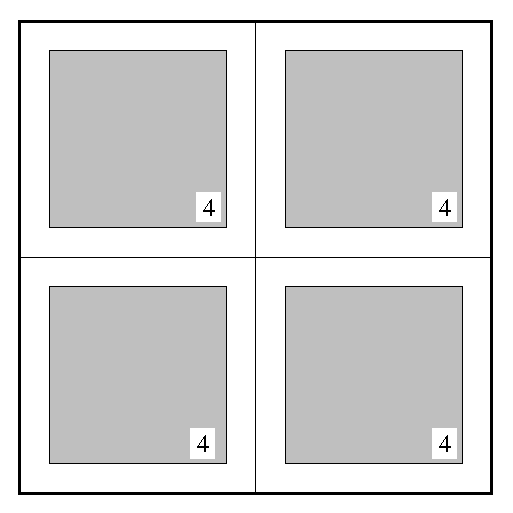
\includegraphics[width=1.8in]{amr2-2.eps} \ \
            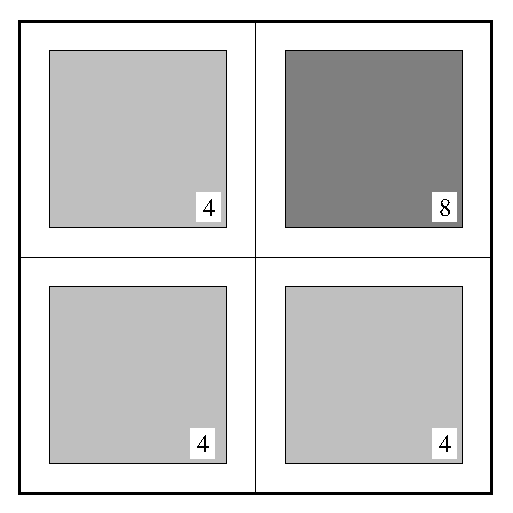
\includegraphics[width=1.8in]{amr2-3.eps}}
\ \\
\centerline{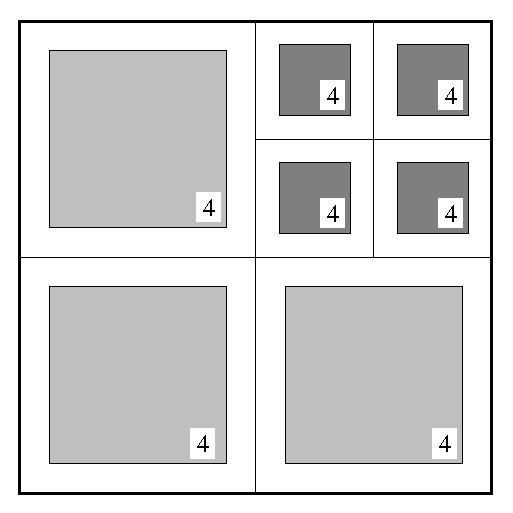
\includegraphics[width=1.8in]{amr2-4.eps} \ \
            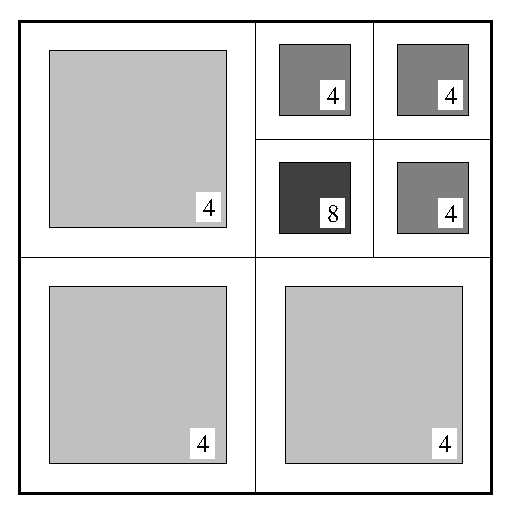
\includegraphics[width=1.8in]{amr2-5.eps} \ \
            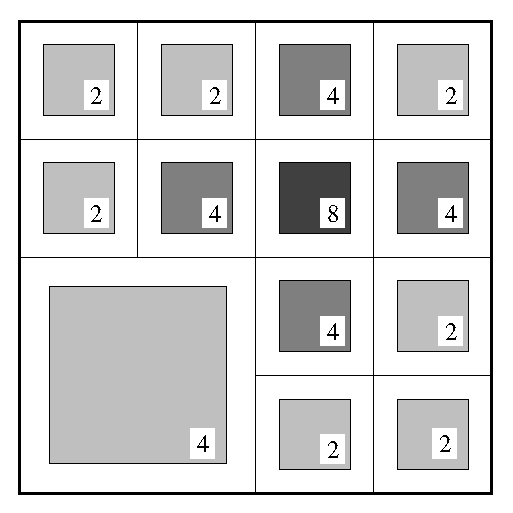
\includegraphics[width=1.8in]{amr2-7.eps}}
\ \\
\centerline{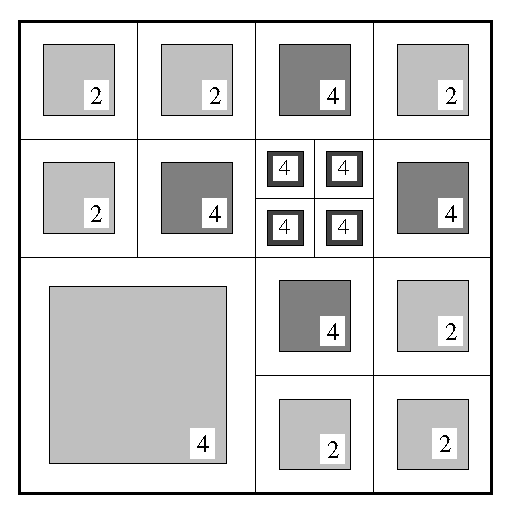
\includegraphics[width=1.8in]{amr2-8.eps} \ \
            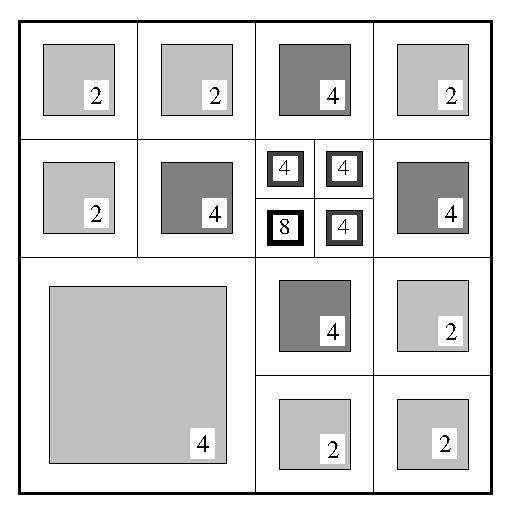
\includegraphics[width=1.8in]{amr2-9.eps} \ \
            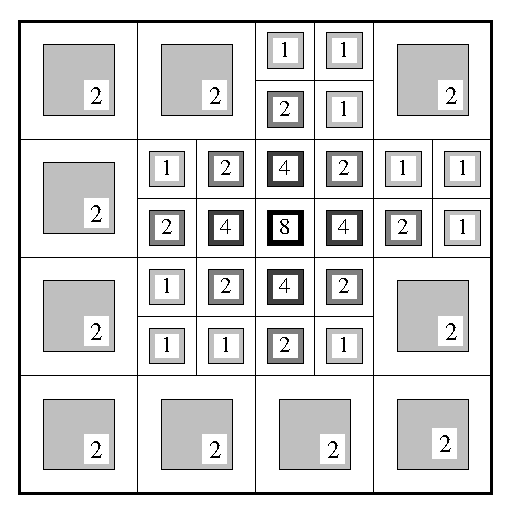
\includegraphics[width=1.8in]{amr2-11.eps}}

%-----------------------------------------------------------------------
\subsection{Use Cases}
%-----------------------------------------------------------------------
%-----------------------------------------------------------------------
\subsection{Parameters}
%-----------------------------------------------------------------------

%=======================================================================
\section{Particles Component} \label{s:component-particles}
%=======================================================================

Specifies data structures and data structure parameters related
to distributed particles.  

\begin{itemize}
\item min\_group\_size
\item max\_group\_size
\end{itemize}

%-----------------------------------------------------------------------
\subsection{Use Cases}
%-----------------------------------------------------------------------
%-----------------------------------------------------------------------
\subsection{Parameters}
%-----------------------------------------------------------------------


%=======================================================================
\section{Parallel Component} \label{s:component-parallel}
%=======================================================================

Hardware platform parallelism will be considered to be multilevel,
including nodes, processors, and cores.  Computational tasks will be
flexibly organized into hierarchical levels to aid mapping to multiple
hardware parallelization levels, including grid patches, grid patch
subblocks, and multiple simulations.  Task sizes in different levels
will allow flexibility to help optimize granularity for the different
given parallelization level components.

Flexible parallelism paradigms: map parallelism to tasks

Automatic code generation (or other) of parallel tasks to implement
parallelism and optimize performance

Specify parallelism type and parameters.  For example, non-blocking
MPI, MPI-2, hybrid MPI/UPC, performance-related parameters such as
buffer size, etc.

Specifiy parallelism and parameters

Specifiy method for controling parallelism

   parallelization method (MPI buffered/blocking, MPI2 Get)

\begin{itemize}
\item MPI (send/recv and type, one-sided and type, what level)
\item OpenMP (num threads, what level)
\item UPC (num threads, what level)
\item pthreads (num threads, what level)
\item cooperative parallelism
\item levels for each if multiple
\end{itemize}

%-----------------------------------------------------------------------
\subsection{Use Cases}
%-----------------------------------------------------------------------
%-----------------------------------------------------------------------
\subsection{Parameters}
%-----------------------------------------------------------------------

%=======================================================================
\subsection{MPI Send/Recv}

%=======================================================================
\subsection{MPI2 Get}

%=======================================================================
\subsection{OpenMP}

%=======================================================================
\subsection{Collaberative parallelism}

%=======================================================================
\subsection{Pipelining}




%=======================================================================
\section{Performance parameters} \label{s:performance}
%=======================================================================

Performance monitoring and optimization(?) parameters

%-----------------------------------------------------------------------
\subsection{Use Cases}
%-----------------------------------------------------------------------
%-----------------------------------------------------------------------
\subsection{Parameters}
%-----------------------------------------------------------------------

%=======================================================================
\section{Monitor parameters} \label{s:monitor}
%=======================================================================

High-level monitoring of the run at a summary level, such as current
timestep, problem time, wall time, cpu time, etc.

%-----------------------------------------------------------------------
\subsection{Use Cases}
%-----------------------------------------------------------------------
\begin{verbatim}
   monitor {
     type   = html
     amount = verbose
   }
\end{verbatim}
%-----------------------------------------------------------------------
\subsection{Parameters}
%-----------------------------------------------------------------------

%=======================================================================
\section{Output parameters} \label{s:output}
%=======================================================================

Output parameters.

%-----------------------------------------------------------------------
\subsection{Use Cases}
%-----------------------------------------------------------------------

\begin{verbatim}
output { 
   name = "data"
   format = hdf5
   type   = [data, input]
   fields = ["density", "velocity", "temperature"]
   file = ["data-%6s" cycle_number]
   cycle = 0:10:90
   cycle = 100:100:900
   cycle = 1000
}
\end{verbatim}

\begin{verbatim}
output { 
   name      = "restart"
   format    = hdf5
   type      = [data, input]
   fields    = all
   file      = ["restart-%6s" cycle_number]
   time_cpu  = 0.5 # CPU hours
   overwrite = true
   copies    = 2
}
\end{verbatim}

\begin{verbatim}
output { 
   name      = "movie"
   file      = ["movie-%6s" cycle_number]
   time      = :10:
   extract   = x == 12
}
\end{verbatim}


%-----------------------------------------------------------------------
\subsection{Parameters}
%-----------------------------------------------------------------------



%=======================================================================
\section{Recover Component} \label{s:component-recover}
%=======================================================================

Fault tolerance and adaptivity parameters

\begin{itemize}
\item fault tolerance methodology
\item adaptivity
\end{itemize}

%-----------------------------------------------------------------------
\subsection{Use Cases}
%-----------------------------------------------------------------------
%-----------------------------------------------------------------------
\subsection{Parameters}
%-----------------------------------------------------------------------



% %------------------------------------------------------------------------
\begin{frame}[fragile] \frametitle{Software Components: High-level}
\end{frame}
%------------------------------------------------------------------------
\begin{frame}[fragile] \frametitle{Control}
      \begin{itemize}
        \item Task: advance grid patch one timestep
        \item Dependencies: boundary values
        \item Dynamic task scheduling
        \begin{itemize}
          \item No artificial dependencies imposed
          \item Patches in different levels can advance concurrently
          \item CHARM++ would be helpful
        \end{itemize}
      \end{itemize}
\end{frame}

% %------------------------------------------------------------------------
\begin{frame}[fragile] \frametitle{Software Components: AMR data structures}
\end{frame}
%------------------------------------------------------------------------
\begin{frame}[fragile] \frametitle{Software Components: \code{Amr}}
\end{frame}

% %------------------------------------------------------------------------
    \begin{frame}[fragile] \frametitle{Software Components: Hardware}
\end{frame}

% %------------------------------------------------------------------------
    \begin{frame}[fragile] \frametitle{Software Components: AMR data structures}
\end{frame}

% %------------------------------------------------------------------------
    \begin{frame}[fragile] \frametitle{Software Components: AMR data structures}
\end{frame}


%========================================================================
\section{Data Structures}
%========================================================================

%------------------------------------------------------------------------
\subsection{Related AMR applications}
%------------------------------------------------------------------------

%------------------------------------------------------------------------
\begin{frame}[fragile] \frametitle{Chombo: Patch-based AMR}
\begin{minipage}{1.5in}
\centerline{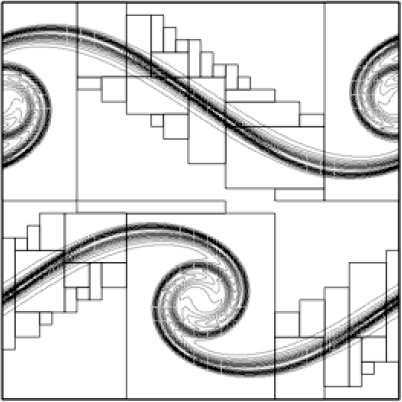
\includegraphics[width=1.5in]{chombo.png}}
\end{minipage} \ 
\begin{minipage}{2.5in}
\begin{itemize}
\enhance{1}\item Colella et al, LBNL
\enhance{2}\item Patch-based with overlayed octree
\enhance{3}\item Parallel grid refinement algorithm
\enhance{4}\item Patches may have multiple parents
\end{itemize}
\end{minipage}
\end{frame}

%------------------------------------------------------------------------
\begin{frame}[fragile] \frametitle{FLASH / Paramesh: Tree-based AMR}
\centerline{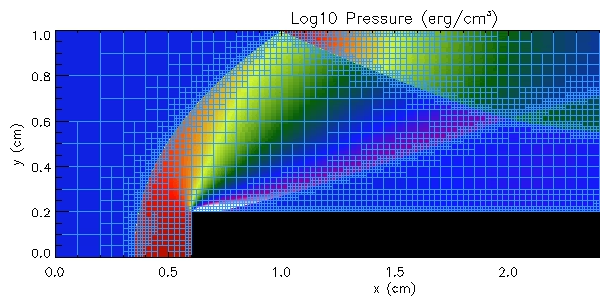
\includegraphics[width=3.0in]{paramesh.png}}
\begin{minipage}{2.3in}
\begin{itemize}
\enhance{1}\item ASCI/Alliance FLASH Center
\enhance{2}\item $>500,000$ lines of code
\enhance{3}\item Uniform time-stepping
\end{itemize}
\end{minipage}
\begin{minipage}{1.8in}
\begin{itemize}
\enhance{4}\item $2^d$-tree refinement 
\enhance{5}\item Fixed-sized patches
\enhance{6}\item No ``level-jumps''
\end{itemize}
\end{minipage}

\end{frame}

% \end{minipage} \
% \begin{minipage}{2in}
% \begin{itemize}
% \enhance{2}\item[+] Easier grid generation
% \enhance{3}\item[+] Fast neighbor search
% \enhance{4}\item[+] Easier to load balance
% \enhance{5}\item[+] Regularly-sized grids
% \end{itemize}
% \end{minipage} \
% \begin{minipage}{2in}
% \begin{itemize}
% \enhance{6}\item[-] More grid patches
% \enhance{7}\item[-] Small grid patches
% \end{itemize}
% \end{minipage}
% 
% \end{frame}

%------------------------------------------------------------------------
\begin{frame}[fragile] \frametitle{\cello: Hybrid Patch-AMR and Tree-AMR}

\begin{minipage}{2in}
\begin{itemize}
\enhance{1}\item Patch-based AMR ala Chombo
\enhance{2}\item Modified tree-based AMR ala FLASH
\begin{itemize}
\enhance{3}\item patch-reduction
\enhance{4}\item child-based refinement
\enhance{5}\item $k^d$-trees
\end{itemize}
\enhance{6}\item Code reuse between patch- and tree-AMR
\end{itemize}
\end{minipage}
\begin{minipage}{2.0in}
\centerline{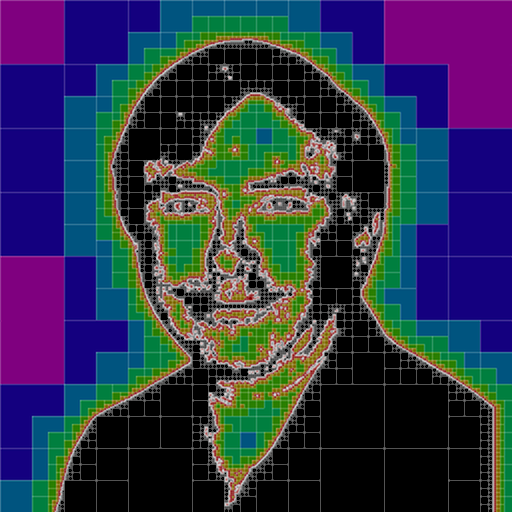
\includegraphics[width=2.0in]{norman.png}}
\end{minipage}
\end{frame}

%------------------------------------------------------------------------
    \begin{frame}[fragile] \frametitle{Review of AMR Applications}
    \footnotesize
      \begin{tabular}{|l|ccc|cc|}
\hline
    &  \textbf{Enzo} & \textbf{Chombo} & \textbf{FLASH} & \textbf{Cello-patch} & \textbf{Cello-tree} \\  \hline
    \textbf{Refinement} &  \enhanceus{2}{patch} & \enhancethem{3}{patch} &  \enhancethem{4}{$2^d$-tree} & \enhancenewus{5}{patch} & \enhancenewus{6}{$k^d$-tree}  \\
%    \textbf{Tree type} & \enhanceus{2}{none} & \enhancethem{3}{octree} & \enhancethem{4}{octree} & \enhancenewus{5}{octree} & \enhancenewus{6}{octree++} \\  \hline
    \textbf{Patch shape} & \enhanceus{2}{  variable} & \enhancethem{3}{variable} &  \enhancethem{4}{constant} & \enhancenewus{5}{variable} & \enhancenewus{6}{constant} \\
    \textbf{Patch size} & \enhanceus{2}{  variable} & \enhancethem{3}{variable} &  \enhancethem{4}{constant} & \enhancenewus{5}{variable} &\enhancenewus{6}{limited}  \\ \hline
    \textbf{Parents} & \enhanceus{2}{single} & \enhancethem{3}{multiple} & \enhancethem{4}{single} &   \enhancenewus{5}{multiple} & \enhancenewus{6}{single} \\
    \textbf{Children} & \enhanceus{2}{variable} & \enhancethem{3}{variable} & \enhancethem{4}{constant} & \enhancenewus{5}{variable} & \enhancenewus{6}{limited} \\
    \textbf{Neighbors} & \enhanceus{2}{variable} & \enhancethem{3}{variable} & \enhancethem{4}{limited} & \enhancenewus{5}{variable} & \enhancenewus{6}{limited} \\\hline
    \textbf{Level jumps} & \enhanceus{2}{ yes} &    \enhancethem{3}{no} &      \enhancethem{4}{no}    &   \enhancenewus{5}{no} & \enhancenewus{6}{no} \\
    \textbf{Asymmetric} & \enhanceus{2}{yes} &  \enhancethem{3}{no} &  \enhancethem{4}{no} &  \enhancenewus{5}{no} & \enhancenewus{6}{no} \\\hline
      \end{tabular}
\end{frame}


%------------------------------------------------------------------------
\subsection{Cello AMR and Arrays}
%------------------------------------------------------------------------

%------------------------------------------------------------------------
\begin{frame}[fragile] \frametitle{\cello\ AMR Philosophy}
\begin{itemize}
\enhance{1}\item Use arrays in uniform resolution regions
\enhance{2}\item Use AMR where resolution changes
\enhance{3}\item Issues with standard tree-based AMR
\begin{itemize}
\enhance{4}\item[a] Lots of small patches at finest resolution
\enhance{5}\item[b] Want ``steeper'' refinement for deep AMR
\end{itemize}
\enhance{6}\item Three proposed modifications:
\begin{enumerate}
\enhance{7}\item Patch coalescing (a)
\enhance{7}\item Individual child refinement (a)
\enhance{7}\item Higher-order refinement with backfill (b)
\end{enumerate}
\enhance{8}\item \code{Array} and \code{Amr} C++ class hierarchies
\end{itemize}
\end{frame}




%----------------------------------------------------------------------
\begin{frame}
\frametitle{Cello Arrays}

\begin{itemize}
\item Conceptually a Fortran-like array
\item Data distributed via MPI-[12], OMP, [UPC]
\item Data layout may be blocked / padded for cache
\item Interface between high-level C++ and low-level Fortran/C
\end{itemize}
\end{frame}

%----------------------------------------------------------------------
\begin{frame}
\frametitle{Cello Array variations}

\begin{minipage}{1.8in}
\begin{itemize}
\item[]\enhance{1-}
\includegraphics[width=0.4in]{array-serial.png} \ \ \code{ArraySerial}
\item[]\enhance{2-}
\includegraphics[width=0.4in]{array-block.png} \ \ \code{ArrayBlock}
\item[]\enhance{3-}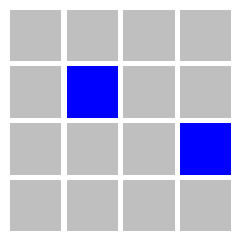
\includegraphics[width=0.4in]{array-mpi.png} \ \ \code{ArrayMpi}
\end{itemize}
\end{minipage} \ 
\begin{minipage}{2in}
\begin{itemize}
\item[]\enhance{4-}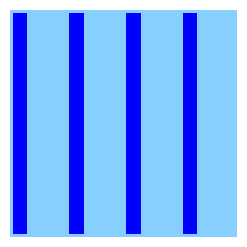
\includegraphics[width=0.4in]{array-omp.png} \ \ \code{ArrayOmp}
\item[]\enhance{5-}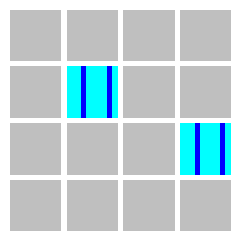
\includegraphics[width=0.4in]{array-mpi-omp.png} \ \ \code{ArrayMpiOmp}
\item[]\enhance{6-}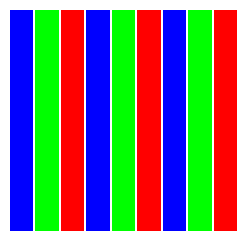
\includegraphics[width=0.4in]{array-interleave.png} \ \ \code{ArrayInterleave}
\end{itemize}
\end{minipage}

\end{frame}
%----------------------------------------------------------------------

\begin{frame}[fragile] \frametitle{Cello AMR: Patch Coalescing}
\centerline{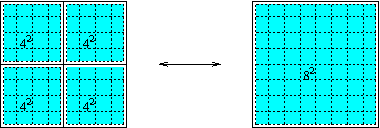
\includegraphics[width=2.5in]{coalesce.png}}
\begin{itemize}
\enhance{2}\item Replace AMR nodes with larger arrays when possible
\enhance{3}\item Replace arrays with AMR nodes when necessary
\enhance{4}\item Allows adapting to constant versus changing resolution
\end{itemize}
\end{frame}

\begin{frame}[fragile] \frametitle{Cello AMR: Individual Child Refinement}
\centerline{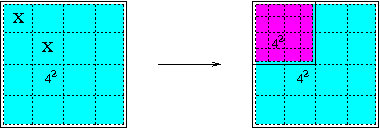
\includegraphics[width=2.5in]{amr-child.png}}
\begin{itemize}
\enhance{1}\item Refine children individually instead of all or nothing
\enhance{2}\item Added flexibility can reduce AMR tree size
\end{itemize}
\end{frame}

\begin{frame}[fragile] \frametitle{Cello AMR: $k^d$ Refinement with Backfill}
\centerline{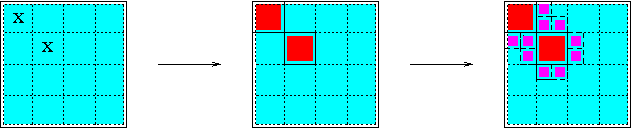
\includegraphics[width=3.5in]{kd-backfill.png}}
\begin{itemize}
\enhance{1}\item If $k=4$, refine by $4$ instead of $2$
\enhance{2}\item More ``targeted'' refinement
\enhance{3}\item Can optionally remove level jumps by ``backfilling'' levels
\enhance{4}\item Backfill patch locations are known implicitly---nominal storage
\enhance{5}\item Many child nodes implies sparse storage
\end{itemize}
\end{frame}


%------------------------------------------------------------------------
\subsection{Point-source tree-AMR example}
%------------------------------------------------------------------------

%------------------------------------------------------------------------
    \begin{frame}[fragile] \frametitle{Point-source test: $2^d$-trees}
\begin{minipage}{2.3in}
\includegraphics<1>[width=2.3in]{dots.png}
\includegraphics<2>[width=2.3in]{dots-4-0.png}
\includegraphics<3>[width=2.3in]{dots-4-1.png}
\includegraphics<4>[width=2.3in]{dots-4-2.png}
\end{minipage}
\begin{minipage}{1.6in}
\footnotesize
      \begin{itemize}
        \item \ENHANCE{1}Test problem: refine on point sources
        \item \ENHANCE{2}Simple quad-tree has level jumps
        \item \ENHANCE{3}After normalization issues remain:
        \begin{itemize}
\footnotesize
          \item \ENHANCE{3}numerous patches
          \item \ENHANCE{3}gradual refinement
        \end{itemize}
        \item \ENHANCE{4}Patch coalescing reduces patch count
      \end{itemize}
\end{minipage} \\
\begin{minipage}{4.0in}
\footnotesize
Nodes: 
\ENHANCE{2}549
\ENHANCE{3}2137
\ENHANCE{4}\textbf{1073}
\color{lightgray}155
\color{lightgray}650
\color{lightgray}\textbf{650}
\color{lightgray}86
\color{lightgray}158
\color{lightgray}\textbf{158}
\end{minipage}
\end{frame}

%------------------------------------------------------------------------
    \begin{frame}[fragile] \frametitle{Point-source test: $2^k$-trees with child-refinement}
\begin{minipage}{2.3in}
\includegraphics<1>[width=2.3in]{dots-4-3.png}
\includegraphics<2>[width=2.3in]{dots-4-4.png}
\includegraphics<3>[width=2.3in]{dots-4-5.png}
\end{minipage} \
\begin{minipage}{1.6in}
\footnotesize
      \begin{itemize}
        \item \ENHANCE{1}Individual child refinement
        \item \ENHANCE{2}Normalize for level jumps
        \item \ENHANCE{3}Patch coalescing not effective
      \end{itemize}
\end{minipage} \\
\begin{minipage}{4.0in}
\footnotesize
Nodes: 
\color{gray}549
\color{gray}2137
\color{gray}\textbf{1073}
\ENHANCE{1}155
\ENHANCE{2}650
\ENHANCE{3}\textbf{650}
\color{lightgray}86
\color{lightgray}158
\color{lightgray}\textbf{158}

\end{minipage}
\end{frame}

%------------------------------------------------------------------------

    \begin{frame}[fragile] \frametitle{Point-source test: $4^d$-trees with child-refinement}
\begin{minipage}{2.3in}
\includegraphics<1>[width=2.3in]{dots-16-3.png}
\includegraphics<2>[width=2.3in]{dots-16-4.png}
\includegraphics<3>[width=2.3in]{dots-16-5.png}
\includegraphics<4>[width=2.3in]{dots-16-5.png}
\end{minipage} \
\begin{minipage}{1.6in}
\footnotesize
      \begin{itemize}
        \item \ENHANCE{1}Refinement by $4$
        \item \ENHANCE{2}Normalize for ($r=4$) level jumps
        \item \ENHANCE{3}Patch coalescing not effective
        \item \ENHANCE{4}Best result:
      \begin{itemize}
\footnotesize
        \item \ENHANCE{4}Fewer patches
	\item \ENHANCE{4}Steep refinement
        \item \ENHANCE{4}Can 'backfill' to regain $r=2$
      \end{itemize}
      \end{itemize}
\end{minipage}
\begin{minipage}{4.0in}
\footnotesize
Nodes: 
\color{gray}549
\color{gray}2137
\color{gray}\textbf{1073}
\color{gray}155
\color{gray}650
\color{gray}\textbf{650}
\ENHANCE{1}86
\ENHANCE{2}158
\ENHANCE{3-4}\textbf{158}

\end{minipage}
\end{frame}

%------------------------------------------------------------------------
\subsection{Cosmology tree-AMR example}
%------------------------------------------------------------------------
%------------------------------------------------------------------------

    \begin{frame}[fragile] \frametitle{Cosmology test: $2^d$-trees}
\begin{minipage}{2.3in}
\includegraphics<1>[width=2.3in]{cosmo2.png}
\includegraphics<2>[width=2.3in]{cosmo2-4-0.png}
\includegraphics<3>[width=2.3in]{cosmo2-4-1.png}
\includegraphics<4>[width=2.3in]{cosmo2-4-2.png}
\end{minipage} \
\begin{minipage}{1.6in}
\footnotesize
      \begin{itemize}
        \item \ENHANCE{1}Test problem: 2D cosmology image
        \item \ENHANCE{2}Basic $2^d$ tree
        \item \ENHANCE{3}Normalize for level jumps
        \item \ENHANCE{4}Coalesce patches
      \end{itemize}
\end{minipage}
\begin{minipage}{4.0in}
\footnotesize
Nodes:
\ENHANCE{2}61261
\ENHANCE{3}81701
\ENHANCE{4}\textbf{32529}
\color{lightgray}35608
\color{lightgray}43950
\color{lightgray}\textbf{35942}
\color{lightgray}33542
\color{lightgray}33868
\color{lightgray}\textbf{31708}
\end{minipage}
\end{frame}

%------------------------------------------------------------------------

    \begin{frame}[fragile] \frametitle{Cosmology test: child-refinement}
\begin{minipage}{2.3in}
\includegraphics<1>[width=2.3in]{cosmo2-4-3.png}
\includegraphics<2>[width=2.3in]{cosmo2-4-4.png}
\includegraphics<3>[width=2.3in]{cosmo2-4-5.png}
\end{minipage} \
\begin{minipage}{1.6in}
\footnotesize
      \begin{itemize}
        \item \ENHANCE{1}Refine on subset of children
        \item \ENHANCE{2}Normalize for level jumps
        \item \ENHANCE{3}Coalesce patches
      \end{itemize}
\end{minipage}
\begin{minipage}{4.0in}
\footnotesize
Nodes:
\color{gray}61261
\color{gray}81701
\color{gray}\textbf{32529}
\ENHANCE{1}35608
\ENHANCE{2}43950
\ENHANCE{3}\textbf{35942}
\color{lightgray}33542
\color{lightgray}33868
\color{lightgray}\textbf{31708}
\end{minipage}
\end{frame}
%------------------------------------------------------------------------

    \begin{frame}[fragile] \frametitle{Cosmology test: $4^d$-trees + child-refinement}
\begin{minipage}{2.3in}
\includegraphics<1>[width=2.3in]{cosmo2-16-3.png}
\includegraphics<2>[width=2.3in]{cosmo2-16-4.png}
\includegraphics<3>[width=2.3in]{cosmo2-16-5.png}
\end{minipage} \
\begin{minipage}{1.6in}
\footnotesize
      \begin{itemize}
        \item \ENHANCE{1}$4^d$-tree refinement
        \item \ENHANCE{2}Normalize for level jumps
        \item \ENHANCE{3}Coalesce patches
      \end{itemize}
\end{minipage}
\begin{minipage}{4.0in}
\footnotesize
Nodes:
\color{gray}61261
\color{gray}81701
\color{gray}\textbf{32529}
\color{gray}35608
\color{gray}43950
\color{gray}\textbf{35942}
\ENHANCE{1}33542
\ENHANCE{2}33868
\ENHANCE{3}\textbf{31708}
\end{minipage}
\end{frame}


%========================================================================
\section{Issues and Solutions}
%========================================================================
%%------------------------------------------------------------------------
\begin{frame}[fragile] \frametitle{Random Sampling of Half-baked Ideas}
      \begin{itemize}
        \item Dynamic scheduling
        \item Time-stepping
        \item Particle positions
        \item Load balancing
        \item Software resiliency
        \item Quality control
      \end{itemize}
\end{frame}

%------------------------------------------------------------------------
\subsection{Dynamic scheduling}
%------------------------------------------------------------------------
%------------------------------------------------------------------------
\begin{frame}[fragile] \frametitle{CHARM++ dynamic scheduling}
\begin{itemize}
\enhance{1}\item ``Machine independent parallel programming system''
\enhance{2}\item Benefits:
\begin{itemize}
\enhance{2}\item Dynamically schedules tasks
\enhance{3}\item Latency tolerant (message-driven execution)
\enhance{4}\item Computation / communication overlap
\enhance{5}\item Dynamic load-balancing
\end{itemize} 
\enhance{6}\item Questions:
\begin{itemize}
\enhance{6}\item Can it be an option?
\enhance{6}\item Code changes global or local?
\enhance{6}\item Tolerance of task granularity?
\enhance{6}\item Worth the effort?
\end{itemize}
\end{itemize}
\end{frame}

%------------------------------------------------------------------------
\subsection{Time-stepping}
%------------------------------------------------------------------------
%------------------------------------------------------------------------
    \begin{frame}[fragile] \frametitle{Time-Stepping Optimization 1}
\begin{minipage}{1.3in}
\includegraphics<1->[width=1.3in]{timestep-levels.png}
\end{minipage} \
\begin{minipage}{1.3in}
\includegraphics<2->[width=1.3in]{timestep-dynamic.png}
\end{minipage} \
\begin{minipage}{1.3in}
\includegraphics<5->[width=1.3in]{timestep-uniform.png}
\end{minipage} \
\begin{itemize}
\enhance{1}\item \enzo\ time-stepping proceeds level by level
\enhance{2}\item Levels may proceed concurrently
  \begin{itemize}
  \enhance{3}\item[$+$] Faster if enough parallelism
  \enhance{4}\item[$-$] Reduced parallel efficiency
  \end{itemize}
\enhance{5}\item Uniform time-stepping
  \begin{itemize}
  \enhance{6}\item[$+$] Improved parallel efficiency
  \enhance{6}\item[$+$] Faster if enough parallelism
  \enhance{7}\item[$-$] More overall work
  \end{itemize}
\end{itemize}
\end{frame}

%------------------------------------------------------------------------
    \begin{frame}[fragile] \frametitle{Time-Stepping Optimization 2}
\begin{itemize}
\enhance{1}\item Allow adaptive time-stepping \textit{within} levels
\enhance{2}\item Each patch determines its local time-step
\enhance{3}\item Eliminates global time-step reduction
\enhance{4}\item Well-suited for dynamic scheduling
\begin{itemize}
\enhance{4}\item Dependencies are local: neighboring patches
\end{itemize}
\enhance{5}\item Quantize time steps to powers of two for alignment
\end{itemize}
\end{frame}

%------------------------------------------------------------------------
\subsection{Particle positions}
%------------------------------------------------------------------------
%------------------------------------------------------------------------
\begin{frame}[fragile] \frametitle{Particle positions}
      \begin{itemize}
        \item Particles are associated with a patch
        \item Represent particles in patch-local coordinates
        \item Simple coordinate transformation when particles migrate
        \item Single-precision sufficient
        \item Global coordinates
      \end{itemize}
\end{frame}
%------------------------------------------------------------------------
    \begin{frame}[fragile] \frametitle{Precision issues: Particles}
      \begin{itemize}
        \item Use local coordinate system when possible
        \begin{itemize}
          \item Particles coordinates [0:1] in containing grid patch
          \item Simple coordinate transform when containing patch changes
          \item Single precision sufficient
          \begin{itemize}
            \item Save memory
            \item Save time
          \end{itemize}
        \end{itemize}
      \end{itemize}
\end{frame}

%------------------------------------------------------------------------
\subsection{Load balancing}
%------------------------------------------------------------------------
%------------------------------------------------------------------------
    \begin{frame}[fragile] \frametitle{Hierarchical Load balancing}
\end{frame}

%%------------------------------------------------------------------------
    \begin{frame}[fragile] \frametitle{Precision issues: Grids}
      \begin{itemize}
        \item Define grid location only relative to neighboring grid
        \item 32-bit integers always sufficient
        \item No global tree structure
        \item Issues
        \begin{itemize}
          \item Load balancing
          \begin{itemize}
            \item CHARM++
          \end{itemize}
          \item Re-gridding
          \begin{itemize}
            \item local algorithm
          \end{itemize}
          \item Global time step
        \end{itemize}
        \item High scalability
      \end{itemize}
\end{frame}

%%------------------------------------------------------------------------
    \begin{frame}[fragile] \frametitle{Gravity}
      \begin{itemize}
        \item Hypre insufficient
        \begin{itemize}
          \item Best method FAC is unusable
        \end{itemize}
        \item Write own FAC
        \item Chombo group is on top of this
      \end{itemize}
\end{frame}

%------------------------------------------------------------------------
\subsection{Software resiliency}
%------------------------------------------------------------------------
%------------------------------------------------------------------------
\begin{frame}[fragile] \frametitle{Software Resiliency}
\begin{itemize}
\enhance{1}  \item Handle software / hardware errors gracefully
  \begin{itemize}
\enhance{2}     \item Identify problems: memory error, node crash, etc.
\enhance{3}     \item Bactrack and continue on reduced hardware
  \end{itemize}
\enhance{4}  \item Use checkpoint/restart library, e.g.~BLCR
\enhance{5}  \item Application / library determines best checkpoint frequency
\enhance{6}  \item Minimize size of checkpoint dumps
  \end{itemize}
\end{frame}

%------------------------------------------------------------------------
%\subsection{Software quality}
%------------------------------------------------------------------------
%%------------------------------------------------------------------------
\begin{frame}[fragile] \frametitle{Software Quality}
\begin{itemize}
  \item Testing finds $90\%$ bugs
  \item Code reviews find $90\%$ bugs
  \item Testing + reviews find $99\%$ bugs
\end{itemize}
\end{frame}


%========================================================================
\section{Conclusions}
%========================================================================

%------------------------------------------------------------------------
\begin{frame}[fragile] \frametitle{Conclusions}
\begin{itemize}
\item \textcolor{blue}{\url{http://client65-88.sdsc.edu/projects/cello}}
\begin{itemize}
\item Testing
\item Features (``Wish List'' wiki or ticket)
\item Parameters (``Parameters'' wiki)
\end{itemize}
\item Reviewing code
\item Contributing code
\end{itemize}
\end{frame}


\end{document}
